\documentclass[a4paper, 11pt]{article}
\usepackage[catalan]{babel}
\usepackage[left=3cm,right=3cm,top=2cm,bottom=2cm]{geometry}
\usepackage{biblatex, csquotes}
\usepackage{amsmath, amssymb}
\usepackage{float, graphicx}
\usepackage{bookmark}

\addbibresource{l01.bib}

\hypersetup{
  colorlinks=true,
  citecolor=magenta,
  linkcolor=blue,
  urlcolor=cyan,
  pdftitle={Interpretació geomètrica de YBC6967},
  pdfpagemode=FullScreen,
}

\title{Interpretació geomètrica del problema de recíprocs de YBC6967}
\author{
  Carlo Sala Gancho\\
  Història de les Matemàtiques\\
  Grau de Matemàtiques\\
  Universitat Autònoma de Barcelona } \date{Febrer 2023}

\begin{document}
\maketitle
\subsection*{Enunciat del problema}
La tauleta YBC6967 ens proposa el seguent problema: \textbf{Un número excedeix el seu recíproc en 7 unitats. Quins són
  els números?} A partir d'aquí, ens proposa la següent solució:
\begin{enumerate}
  \item Parteix en dues meitats el $7$, i obtindràs $3;30$.
  \item Multiplica $3;30$ per $3;30$ i obtindràs $12;15$.\label{pas}
  \item Afegeix $1$ al $12;15$ que havies obtingut i obtindràs $1\ 12;15$.
  \item Quin és el costat del quadrat $1\ 12;15$? $8;30$.
  \item Substreu $3;30$, el \textit{quadrat-talkitum} de $8;30$ i després afegeix-lo a $8;30$.
  \item Un és $12$ i l'altre $5$. El recíproc és $12$, i el seu recíproc és $5$.
\end{enumerate}

Aquest problema, i especialment la seva resolució, ens fa pensar en com resolien els problemes els babilonis. En efecte
(i aquí ja entrem en conjectures d'historiador), sembla que hi havia un gran fonament geomètric darrere de les
conclusions a les que arribaven. Vegem-ne un exemple molt i\lgem{}ustratiu amb aquesta tauleta.
Observant~\ref{fig:proc}, comprenem quin és el procediment utilitzat per obtenir el costat del rectangle. L'objectiu
sembla ser provar de construir un quadrat d'àrea més gran que el rectangle original, del qual en coneixem el costat (o
bé l'àrea), per poder aconseguir els dos costats del rectangle. En efecte, en el pas~\ref{pas} el que fa es construir
un quadrat de costat $3;30$ (que a la imatge surt amb àrea $12;15$). Just després, retalla el rectangle de la dreta i
el mou a sota a l'esquerra. Ja hem construit, aleshores, un quadrat amb àrea coneguda $60;00 + 12;15$ el qual en podem
aconseguir el costat. Aquest costat, per com hem construit el quadrat, és $3;30$ + la longitud que volem conèixer.

Aquest mètode de construir quadrats de costat conegut per deduir-ne mesures desconegudes és una constant en diverses
tauletes de matemàtiques babilòniques. Això fa veure com aquesta civilització va construir les seves matemàtiques a
partir de l'entorn que els envoltava, i les seves necessitats de cada moment. Avui en dia, en canvi, les matemàtiques
van molt per davant de la nostra percepció de l'entorn. Sense anar més enllà, treballem habitualment amb geometria en
l'espai $\mathbb{R}^4$, quan realment només som capaços de percebre fins a $\mathbb{R}^3$. És realment curiós com hem
fet evolucionar les matemàtiques des d'aquell moment. Tanmateix, en aquest curt assaig no tenim espai per parlar-ne.

Hi ha un petit detall que salta a la vista i, sens dubte, fa pensar. Hi ha un moment del procediment, en el que tenim
un quadrat d'àrea $1\ 12;15$, i volem obtenir-ne el seu costat. Això planteja un problema del tipus $x^2 = K$, una
arrel quadrada. Com aconseguien fer arrels quadrades? Per tauletes que hem recuperat, sabem que tenien taules de
recíprocs, però com els obtenien en primera instància? La teoria més versemblant sembla ser que simplement provaven, i
obtenien aproximacions a base de llapis i paper (o argila i punxó, més aviat). No deixa de ser notable que una
civilització tan antiga com ho eren els babilonis es dediquessin a fer aproximacions d'arrels quadrades amb la precisió
amb la que ho feien (veure YBC 7289, per una aproximació sorprenentment precisa de $\sqrt{2}$), cosa que, fins fa no
massa dies que els computadors van entrar en joc, nosaltres també feiem.

La civilització babilònica va estar molt avançada en la seva època a nivell matemàtic, especialment comparat amb la
civilització egípcia. La manera com resolien els problemes era molt particular, i especialment interessant
d'investigar. Es una pena que ens quedin tan pocs documents d'aquella època per poder conèixer-los encara millor.

\begin{figure}[H]
  \centering
  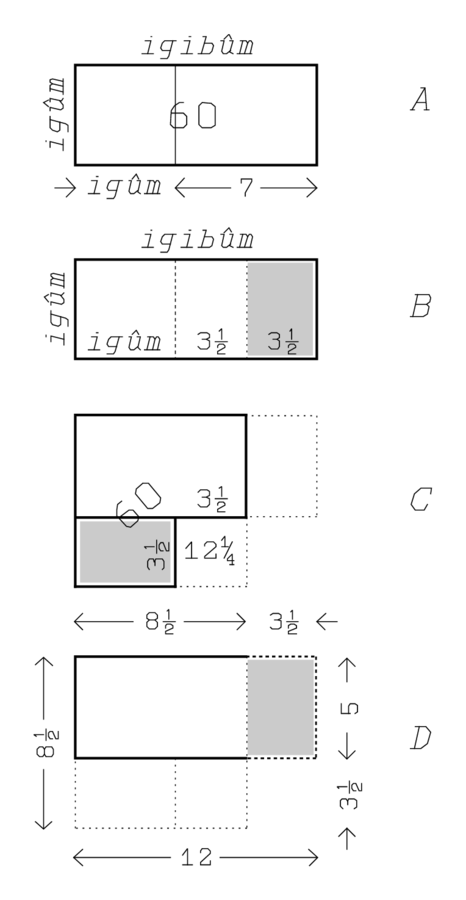
\includegraphics[width=5cm]{figura1.png}
  \caption{Procediment de YBC6967}\cite{bib:fig:proc}\label{fig:proc}
\end{figure}

\printbibliography{}
\end{document}
